\documentclass[american,titlepage]{ntnuthesis}
\usepackage{todonotes}
\usepackage{multirow}
\usepackage{chngpage}
\title{What Do We Know About Operationalizing Machine Learning Models? A Systematic Literature Review.}
\shorttitle{DevOps for AI}
\author{Ask Berstad Kolltveit}
\shortauthor{CoPCSE$@$NTNU}


\addbibresource{thesis.bib}
\addbibresource{review.bib}

% From https://www.overleaf.com/learn/latex/Glossaries

\makeglossaries % Prepare for adding glossary entries


\newglossaryentry{latex}
{
        name=latex,
        description={Is a mark up language specially suited for
scientific documents}
}

\newglossaryentry{bibliography}
{
        name=bibliography,
        plural=bibliographies,
        description={A list of the books referred to in a scholarly work,
typically printed as an appendix}
}

\newglossaryentry{maths}
{
    name=mathematics,
    description={Mathematics is what mathematicians do}
}

\newglossaryentry{technical_debt}{
    name={technical debt}, 
    description={Software engineering term for the degradation of code quality that occurs over time as a software system is developed and evolved}
    }

% --------------------
% ----- Acronyms -----
% --------------------

\newacronym{phd}{PhD}{philosophiae doctor}
\newacronym{CoPCSE}{CoPCSE@NTNU}{Community of Practice in Computer ScienceEducation at NTNU}
\newacronym{gcd}{GCD}{Greatest Common Divisor}
\newacronym{slr}{SLR}{systematic literature review}
\newacronym{glr}{GLR}{grey literature review}
\newacronym{sms}{SMS}{systematic mapping study}
\newacronym{mlr}{MLR}{multivocal literature review}
\newacronym{gl}{GL}{grey literature}
\newacronym{wl}{WL}{white literature}
\newacronym{se}{SE}{software engineering}
\newacronym{ml}{ML}{machine learning}
\newacronym{ai}{AI}{Artificial Intelligence}
\newacronym{ci}{CI}{continuous integration}
\newacronym{cd}{CD}{continuous deployment}
\newacronym{cde}{CDE}{continuous delivery}
\newacronym{ka}{KA}{knowledge area}
\newacronym{slo}{SLO}{service level objective}
\newacronym{rq}{RQ}{research question}
\newacronym{rpc}{RPC}{remote procedure call}
\newacronym{rest}{REST}{representational state transfer}
\newacronym{api}{API}{application programming interface}
\newacronym{kpi}{KPI}{key performance indicator}
\newacronym{iot}{IoT}{Internet of Things}
\newacronym{cpu}{CPU}{central processing unit}
\newacronym{gpu}{GPU}{graphics processing unit}
\newacronym{tpu}{TPU}{tensor processing unit}
\newacronym{mlaas}{MLaaS}{machine learning-as-a-service}
\newacronym{io}{IO}{input/output} % add glossary and acronym lists before document

\begin{document}

\chapter*{Abstract}
Deploying \acrfull{ml} models to production with the same level of rigor and automation as traditional software systems has shown itself to be a non-trivial task, requiring extra care and infrastructure to deal with the additional challenges.
This study is a systematic literature review investigating the state of the art in operationalizing \acrshort{ml} models using the following research questions.
\begin{itemize}
    \item \textbf{RQ1: How are \acrshort{ml} models operationalized in the state of the art?}
    \item \textbf{RQ2: What are the main challenges in operationalizing \acrshort{ml} models?}
    \item \textbf{RQ3: What tools and software infrastructure are used to operationalize \acrshort{ml} models?}
    \item \textbf{RQ4: What are the feature gaps in the tooling and infrastructure used to operationalize \acrshort{ml} models?}
\end{itemize}
The results of the review show that there are many different techniques for operationalizing ML models, and there exists a number of tools for the most common use cases, cloud deployment in particular. 
The review also revealed several opportunities for research into better tooling and infrastructure, particularly for serving and edge \acrshort{ml} deployments.
The results of the study should provide a better overview of different deployment approaches and architectures than previous reviews on the topic, as well as giving an overview of some of the tooling used and opportunities for future research.
% \chapter*{Sammendrag}

Dokumentklassen \texttt{ntnuthesis} er en tilpasset versjon av \LaTeX' standard \texttt{report}-klasse. Den er tilrettelagt for avhandlinger på alle nivåer – bachelor, master og PhD – og er tilgjengelig på både norsk (bokmål og nynorsk) og engelsk (britisk og amerikansk). Dette dokumentet er ment å tjene (i) som en beskrivelse av dokument\-klassen, (ii) som et eksempel på bruken av den, og (iii) som en mal for avhandlingen.


\tableofcontents
\listoffigures
\listoftables
% \lstlistoflistings

\printglossary[type=\acronymtype] % Print acronyms
\printglossary                    % Print glossary
\chapter{Introduction}

Over the years, several thesis templates for \LaTeX{} have been developed by different groups at NTNU. Typically, there have been local templates for given study programmes, or different templates for the different study levels – bachelor, master, and \acrshort{phd}.\footnote{see, e.g., \url{https://github.com/COPCSE-NTNU/bachelor-thesis-NTNU} and \url{https://github.com/COPCSE-NTNU/master-theses-NTNU}}

Based on this experience, the \acrfull{CoPCSE}\footnote{\url{https://www.ntnu.no/wiki/display/copcse/Community+of+Practice+in+Computer+Science+Education+Home}} is hereby offering a template that should in principle be applicable for theses at all study levels. It is closely based on the standard \LaTeX{} \texttt{report} document class as well as previous thesis templates. Since the central regulations for thesis design have been relaxed – at least for some of the historical university colleges now part of NTNU – the template has been simlified and put closer to the default \LaTeX{} look and feel.

The purpose of the present document is threefold. It should serve (i) as a description of the document class, (ii) as an example of how to use it, and (iii) as a thesis template.

\chapter{Background}
\label{ch:background}
This chapter will briefly explain status of machine learning today, technical debt in ML systems and motivate the need for MLOps.

\section{Machine Learning}
Adoption of \acrshort{ml} is growing, and is providing value in a wide array of different fields.
\textcite{mckinsey2020} reports that 50\% of businesses surveyed have adopted \acrshort{ai} in some business function.
However, most companies are still in the very early stages of incorporating \acrshort{ml} in their business processes \cite{Schloegl2019}.
\todo[inline]{Add a bit more on adoption of ML. Maybe technology developments.}

\section{Software Engineering for ML systems}
\todo{Add softer introduction..}
ML systems accrue a lot of \gls{technical_debt} according to \textcite{Sculley2015}.
This is because in addition to the technical debt incurred by being a software system, with the usual tech debt associated with code, ML systems also have entangled data dependencies.
The Software Engineering for Machine Learning movement aims to bring already well-established best practices from the SE domain to the field of ML [cite].
\todo{Add some more content.}

\section{DevOps for ML systems -- \emph{MLOps}}
DevOps is a subset of software engineering focused on tightening the coupling between development and operation of software systems.
DevOps principles advocate for process automation [cite], which is often expressed through the use of version control systems, automated build and deploy pipelines, etc [cite].
Some motivating factors for automation are shortening the time to delivery, increasing reproducibility and reducing time spent on automatable processes [cite].
DevOps for Machine Learning, named MLOps, is a subset of SE4ML and a superset/extension of DevOps, focused on adopting DevOps practices when developing and operating ML systems [cite].
This is because existing DevOps practices are not sufficient for ML systems, which pose additional requirements [cite].
ML systems not only have code dependencies, but have data dependencies in addition, which may impose the requirement of data monitoring (for data distributions shift), continuous training or automatic retraining, etc.

\section{Deploying ML systems}
\todo{Not sure if this belongs in the Background chapter. Seems odd to present my area of research as background information.}
The deployment step consists of taking the system from a development environment (e.g. local development machine) to a production environment (e.g. a server).
For traditional software systems, this process has seen widespread adoption of automated integration and deployment pipelines (CI/CD) for many years [cite].
However, the deployment of ML systems has yet to see such widespread use of CI/CD for multiple different reasons:
\begin{itemize}
    \item Model development is usually done by data scientists [cite], who may not be familiar with DevOps practices or tools.
    \item Models are often developed in notebooks, which are usually not readily deployable [cite].
    \item Models may be developed with different programming languages than what is used in the production environment [cite].
\end{itemize}
\chapter{Related Work}
\label{ch:related_work}
Multiple systematic literature studies have already been conducted on the field of Software Engineering for AI/ML.

\textcite{Shahin2017} performed a comprehensive \acrfull{slr} of tools, practices, approaches and challenges for continuous software engineering (\acrshort{ci}/\acrshort{cd}/\acrshort{cde}).
The authors identified thirty approaches and associated tools for facilitating continuous software engineering practices, and found they were being applied in a wide variety of application domains.
The application of the identified approaches to \acrshort{ml} systems is not discussed or mentioned.

\textcite{Rodriguez2017} performed a \acrfull{sms} of \acrshort{cd}, focusing on the state of research, characteristics of \acrshort{cd} and benefits, challenges and gaps in the research.
The authors identify nine concrete areas for future research opportunities, but the topic of applying \acrshort{cd} to \acrshort{ml} is not discussed.

\textcite{Baier2019} surveyed the academic literature for challenges in deploying \acrshort{ml} models.
The authors also conducted eleven semi-structured expert interview with \acrshort{ml} practitioners from a wide variety of industries.
The data from the literature survey and expert interviews were combined and analyzed in order to produce an overview of practical challenges surrounding \acrshort{ml} within the categories of pre-deployment, deployment, and non-technical issues.
The authors found that the practitioners' experiences generally confirmed challenges reported in the academic literature.

\textcite{Paleyes2020} did a survey of case studies on deploying \acrshort{ml} models with the goal of outlining a research agenda for addressing the challenges that practitioners were found to encounter.
The authors identified practical challenges in sixteen different steps of \acrshort{ml} deployment, and suggest further research to be done in the areas of tooling and services for individual challenges, as well as new holistic approaches for dealing with \acrshort{ml} systems engineering.

\textcite{Kumeno2020} performed an \acrshort{slr} of \acrshort{se} challenges for \acrshort{ml}, and mapped them to the twelve \acrfullpl{ka} of the SWEBOK \cite{Bourque2014}.
The author found that challenges in \acrshort{se} for \acrshort{ml} are found in all \acrshortpl{ka}, and that safety/security and non-technical areas in particular have received a lot of attention in the literature.

\textcite{Nascimento2020} performed an \acrshort{slr} of challenges and practices in \acrshort{se} for \acrshort{ml}. The challenges and practices are mapped to the \acrshortpl{ka} of the SWEBOK.
The authors found that studies from laboratory environments are mainly concerned with building and testing models, which could indicate that more literature produced by industry practitioners should be studied when looking to review the state of the art and state of practice of deploying models to production.
This is further illustrated when the authors highlight that deployment is one of the areas with the fewest suggested practices in published literature.

\textcite{Lwakatare2020} conducted an \acrshort{slr} on  \acrshort{se} for \acrshort{ml} using a two-dimensional scheme, categorizing challenges according to quality attributes (adaptability, scalability, privacy and safety) and \acrshort{ml} development workflow step (data acquisition, training, evaluation, deployment).
The authors also identify solutions to some of the challenges, but note that areas such as privacy and safety are missing solutions, as well as areas such as evaluation and deployment.
The exclusion of \acrshort{gl} is mentioned as a threat to validity of the study.

\textcite{Lwakatare2020a} did an exploratory case study on \acrshort{cd} for \acrshort{ml}.
The authors performed an \acrshort{mlr} to create a five-step process improvement conceptual model for the \acrshort{ml} deployment process. 
The results were validated by conducting a focus group with ten \acrshort{ml} practitioners at a telecommunications company.

\textcite{Serban2020} identified 29 best practices of \acrshort{se} for \acrshort{ml} through conducting an \acrshort{mlr}, before conducting a practitioner survey to investigate adoption and impact of the practices.
The authors perform extensive quantitative analysis of the survey responses, investigating the relationships between practice and effect, correlation between practices, and the importance of each practice.

\textcite{Karamitsos2020} perform an \acrshort{slr} in order to propose a CI/CD pipeline for ML systems, providing suggestions for practices and tools to facilitate the pipeline.
However, the paper lacks rigor, reporting no details of the search, study selection, data extraction or data synthesis procedures, and providing no discussion of the results or threats to validity.

\textcite{John2021} performed an \acrshort{mlr} of the SE lifecycle of ML models, outlining challenges and best practices in each step of the lifecycle.
\todo{Summarize better. Add evaluation/critique. Add relation to this paper.}

\textcite{Giray2021} conducted an \acrshort{slr} of \acrshort{se} for \acrshort{ml}, where challenges and solutions were grouped by areas suggested in SWEBOK, similarly to \cite{Kumeno2020} and \cite{Nascimento2020}, while including an even greater number of papers than any previous SLR in the field.

\textcite{Lorenzoni2021} conducted an \acrshort{slr} of \acrshort{ml} model development, identifying phases, techniques, gaps and trends in the \acrshort{ml} development lifecycle.
The deployment aspect is only briefly mentioned.

\textcite{MartinezFernandez2021} performed an extensive \acrshort{sms} of SE4AI.

\todo[inline]{Write about \textcite{Serban2021} (?)}

\todo[inline]{Write about \textcite{John2021a}}

A common characteristic of previous work is that it tends to be quite broad in scope, covering many areas of \acrshort{se} for \acrshort{ml}.
This study will make the following novel contributions to the research.
\begin{itemize}
    \item Focus specifically on the deployment aspect
    \item Focus on tooling
    \item Include \acrshort{gl} as well as \acrshort{wl}
\end{itemize}

\begin{table}[h]
\begin{adjustwidth}{-1in}{-1in}
    \centering
    \begin{tabular}{l c c c c}
        Study & Deployment-focused & Includes \acrshort{gl} & Tooling-focused & Within field of \acrshort{se} for \acrshort{ml} \\
        \hline
        \textcite{Shahin2017} & X & & X & \\
        \textcite{Rodriguez2017} & X & & & \\
        \textcite{Baier2019} & X & & & X \\
        \textcite{Paleyes2020} & X & & & X \\
        \textcite{Kumeno2020} & & & & X \\
        \textcite{Nascimento2020} & & & & X \\
        \textcite{Lwakatare2020} & X & & & X \\
        \textcite{Lwakatare2020a} & X & X & & X \\
        \textcite{Serban2020} & & X & & X \\
        \textcite{Karamitsos2020} & & & & X \\
        \textcite{John2021} & X & X & & X \\
        \textcite{Giray2021} & & & & X \\
        \textcite{Lorenzoni2021} & & & & X \\
        \textcite{MartinezFernandez2021} & & & & X \\
        \textcite{Serban2021} & & & & X \\
        This study & X & X & X & X \\
    \end{tabular}
    \caption{Comparison of related work with this study.}
    \label{tab:related_work_comparison}
\end{adjustwidth}
\end{table}

As can be seen from \cref{tab:related_work_comparison}, \cite{Lwakatare2020a} and \cite{John2021} are the closest competitors to this study.
\chapter{Research Design and Implementation}
\label{ch:research_design_and_implementation}
This chapter will discuss the motivation, design and implementation of the SLR.
The chapter is structured as follows.
In \cref{sec:research_motivation} the impact and usefulness of the study is argued.
\cref{sec:research_questions} presents the research questions of the study.
\cref{sec:research_method} outlines the research method and design of the study.
Finally, \cref{sec:research_implementation} accounts for how the study was conducted.

\section{Research Motivation}
\label{sec:research_motivation}
As outlined in \cref{ch:background}, industry adoption of ML is still in its early stages and rapidly growing.
The SE aspect of ML is an active field of research, with the vast majority of work having been done only in the past five years.
As reported by earlier literature studies in the field (see \cref{ch:related_work}), deployment of ML is an area which presents real challenges to practitioners.
Tackling deployment challenges requires adopting good practices as well as utilizing suitable tooling.
Much of the earlier work has largely had a broad scope, with goals of mapping out broad SE challenges and practices for ML.
Further, earlier work has had a focus on reviewing the academic literature, ignoring the vast body of practitioner knowledge found in the GL.
To summarize, this study is motivated by three factors.
\begin{itemize}
    \item Researching ML deployment specifically, and not as part of a broader study of SE for ML.
    \item Including more practitioner knowledge in the form of GL.
    \item Putting more focus on tooling by identifying what needs are fulfilled by current tooling and what is missing from tooling.
\end{itemize}

\section{Research Questions}
\label{sec:research_questions}
The overarching research question of this study is "\textbf{What is the state of the art and state of the practice in ML deployment?}".
The focus will be on tooling and trying to identify feature gaps reported in studies where model deployment is discussed.
To support the main research question, four subquestions have been formulated:
\begin{itemize}
    \item \textbf{RQ1: How is ML model deployment handled in real-world applications?}
    \item \textbf{RQ2: What are the main challenges and pain points in ML model deployment?}
    \item \textbf{RQ3: What tools are used to deploy ML models?}
    \item \textbf{RQ4: Are there any feature gaps in the tooling used to deploy ML models?}
\end{itemize}


\section{Research Method and Design}
\label{sec:research_method}
This study is a multivocal literature study (MLR) largely based on the guidelines in \textcite{Kitchenham07guidelinesfor} and \textcite{Garousi2019}.

\subsection{Search Strategy}
\subsubsection{White Literature}
Initial string-based searches in digital libraries failed to produce adequately relevant articles for the topic at hand, thus motivating the use of snowballing as an alternative approach for identifying candidate papers.
The snowballing procedure followed the process proposed by \textcite{Wohlin2014}, with the exception of limiting forward and backward snowballing to a single iteration each.

\subsubsection{Grey Literature}
Pilot searches using Google revealed that adequately relevant and recent results were found using the search string "mlops deployment".
Based on the outlined GL search guidelines in \cite{Garousi2016}, the Top N-approach was selected with the search string "mlops deployment" and $N=100$.

\subsection{Study Selection}
\subsubsection{White Literature}
Inclusion criteria for WL:
\begin{itemize}
    \item Written in English
    \item Published in a peer-reviewed journal, conference or workshop
    \item Published after 2010
    \item Discusses one of the following aspects of machine learning deployment: challenges, solutions, tooling, processes, requirements
    \item Available online
\end{itemize}

Exclusion criteria for WL:
\begin{itemize}
    \item One of the inclusion criteria is not satisfied
\end{itemize}

\subsubsection{Grey Literature}
Inclusion criteria for GL:
\begin{itemize}
    \item Written in English
    \item Published after 2010
    \item Discusses one of the following aspects of machine learning deployment: challenges, solutions, tooling, processes, requirements
    \item Available online
\end{itemize}

Exclusion criteria for GL:
\begin{itemize}
    \item One of the inclusion criteria is not satisfied
\end{itemize}

\subsection{Study Quality Assessment}
\subsection{Data Extraction}
In order to answer the research questions, sufficient data must be gathered from the literature.
Thus, the following data extraction form was designed:

\begin{itemize}
    \item Source type (WL/GL)
    \item Publication date
    \item Process
    \begin{itemize}
        \item What was the deployment process?
    \end{itemize}
    \item Tools
    \begin{itemize}
        \item What tools were used for deployment?
        \item What tooling features were used for deployment?
    \end{itemize}
    \item Challenges
    \begin{itemize}
        \item Is any deployment challenge reported?
        \item What was the challenge?
    \end{itemize}
    \item Solutions
    \begin{itemize}
        \item What challenge is addressed?
        \item What is the solution?
        \item Is the solution merely theoretical (proposed), or do the authors implement it?
        \item If the solution was implemented, what was the outcome?
    \end{itemize}
    \item Requirements
    \begin{itemize}
        \item What functional requirements do the authors state for deployment tooling?
        \item What non-functional requirements do the authors state for deployment tooling?
        \item What is the reasoning for the stated requirements?
    \end{itemize}
    \item Gaps
    \item \begin{itemize}
        \item Is any shortcoming in deployment tooling either implicitly or excplicitly reported?
        \item What are the shortcomings?
        \item How was the shortcoming inferred from the literature (by me)?
    \end{itemize}
    \item Other
\end{itemize}

\subsection{Data Analysis}
\subsection{Data Synthesis}

\section{Research Implementation}
\label{sec:research_implementation}
\chapter{Research Results}
This chapter presents the results from the SLR on a per-research question basis.

\section{RQ1: How is ML Model Deployment Handled in the State of the Art?}
\subsection{Packaging and Integration}
Packaging models in containers accessible through REST or RPC interfaces is a commonly reported method of integration, in which the model is wrapped in an API layer \cite{Garcia2020, Li2017, Ruf2021, Crankshaw2017}.
When deploying many models, using a consistent standard for APIs, such as OpenAPI\footnote{\url{https://www.openapis.org/}}, across models can facilitate system integration \cite{Garcia2020}.
Another reported method of integration is to serialize the model (e.g. into ONNX\footnote{\url{https://onnx.ai/}}, HDF5, joblib) and load it at runtime, possibly with an ML framework that is optimized for production (such as caffe2) \cite{Hazelwood2018, Peticolas2019, Paeaekkoenen2020, Chahal2020}.
The model could also be packaged in a format specific to an end-to-end framework such as MLflow \cite{Chen2020}.
The model may be integrated directly into the application code \cite{Liu2020, Ruf2021, Granlund2021}, traditionally first having to be rewritten for production \cite{Hazelwood2018}.

\subsection{Deployment}
Deployment, the transitioning of a  packaged and integrated model into a serving state, may occur through a few different methods.
Models packaged in containers are simply run directly as standalone services \cite{Liu2020,Ruf2021, Granlund2021, Li2017, Garcia2020}.
However, models may be deployed in a target environment that is different from where they are packaged, in which case the model transfer may happen through either a push- or a pull-pattern.

In a pull-pattern deployment, the target environment (host application running on e.g. server or edge device) periodically polls for model updates and downloads when available \cite{Paeaekkoenen2020, Li2017, Peticolas2019}.

In a push-pattern deployment, the target environment is notified of the availability of a new model by a master server, e.g. by the server where the model was trained.
This will happen either through a messaging service \cite{Liu2020, Garcia2020}, where message contains metadata including the location of the updated model, or by the model being pushed directly to the target environment through some receiving interface \cite{Paeaekkoenen2020}.

When an updated model has reached the target environment, subsequent redeployments can happen in a few different ways.
For models packaged as standalone containers, a container orchestration service (e.g. Kubernetes) can roll out updated models without downtime.
Serialized models may simply be loaded into memory by the application, potentially leading to downtime.
If the hosting application is containerized, model redeployment may be orchestrated by deploying a new application instance with the new model data, alongside the old instance.
When the new instance is finished initializing, it can start serving requests, and the old instance may be evicted \cite{Paeaekkoenen2020}.
To avoid high response latencies for the first query (cold-start issues), models may be queried with an empty request (or an explicit warm-up function call may be used if available) which forces lazy-loaded model components to initialize \cite{Li2017}.

When using an ML deployment service (e.g. SageMaker), the service may handle the deployment of serialized models \cite{Chahal2020}.

Models intended for batch predictions may simply be plugged into a computing pipeline such as Apache Spark\footnote{\url{https://spark.apache.org/}}, computing predictions and storing them in a database or data warehouse \cite{Li2017}.

\subsection{Serving and Inference}
Models are commonly made available for serving predictions through a REST \cite{Krishnamurthi2019, Liu2020, Ruf2021, Garcia2020, Crankshaw2017, Paeaekkoenen2020} or RPC \cite{Ruf2021, Li2017, Crankshaw2017} API.
To meet inference SLOs, there are several techniques reported.
One is model-switching, where less accurate but more performant models are used during periods of high load in order to meet required SLOs \cite{Zhang2020}.
Another is to use adaptive batching queues with a timeout, where queries are batched together in batch sizes that are tuned to the individual model and framework. During periods of low traffic, the timeout is reached before the query batch is filled, and inference is run on the batch in order to not exceed the SLO \cite{Crankshaw2017}.
Additionally, a cache layer may be put on top of the model to reduce computation \cite{Crankshaw2017}.
In order to avoid cold-start issues caused by model loading and initialization, models should be warmed up at deployment and be kept perpetually warm over the course of its life \cite{Zhang2020}.
Model warmup can be achieved through either a method provided by the ML framework \cite{Li2017}, or more generally through issuing an empty query against the model \cite{Garcia2020}.

\subsection{Monitoring and Logging}
Runtime monitoring is important for operationalized ML in order to increase trust and detect performance degradations \cite{Rausch2019, Li2017}.
When the model is operational, the whole application stack is constantly monitored for performance metrics such as latency, throughput, disk utilization, et cetera \cite{Ruf2021, Peticolas2019}.
Predictions are logged, and when available joined with actual outcomes\cite{Li2017}.
Model accuracy should be used to determine when a new model is needed \cite{Peticolas2019}.
The application should be validated against predefined KPIs of the project \cite{Ruf2021}.

\section{RQ2: What Are the Main Challenges in ML Model Deployment?}
\todo[inline]{Need to think about how to present RQ2 and RQ3 in relation to RQ1 and RQ4 in order to minimize overlap.}
\subsection{Packaging and Integration}
ML frameworks are not all created equal, and may be better suited for research than production or vice versa, typically because of performance characteristics versus support for rapid experimentation and debugging.
\cite{Crankshaw2017} notes several challenges in deploying ML frameworks: interface inconsistency across frameworks, changes over time in what is the best framework for the job, and frameworks that are not optimized for deployment.
Developers then have to make the choice of either using a suboptimal framework, or incurring technical debt in order to support and integrate multiple frameworks.

\cite{Hazelwood2018} reports solving this tradeoff by decoupling the frameworks from the model by transferring it from research to production using an exchange format for neural networks.
\cite{Crankshaw2017} also uses decoupling as a solution to this problem, but opts for adding an abstraction layer with a simple interface on top of all models.
This solution is more general, as it is not specific to neural networks.

\cite{Bosch2021} reports the extensive use of glue code as a challenge with which companies struggle.
Glue code is code that merely glues together different parts of the program, without itself providing any functionality.
The authors also highlight the integration of data-driven models with computation-driven software components as a potentially non-trivial task.

\subsection{Serving}
Serving-related challenges are some of the most often reported ones in the literature \cite{Bosch2021, Richins2020, Li2017, Baylor2017, Garcia2020, Crankshaw2017, Lwakatare2019, Bernardi2019, Yadwadkar2019, Chahal2020, Choi2021, Zhang2020, Gupta2020}, usually from a performance perspective.

Achieving a low inference latency and high throughput is widely reported as a challenge in serving ML models \cite{Bosch2021, Li2017,Crankshaw2017,Lwakatare2019,Bernardi2019}.
\textcite{Bernardi2019} found that there is a statistically significant negative correlation between latency and conversion rate at Booking.com, highlighting the business impact of serving performance.

Several potential solutions for improving serving performance have been proposed in the literature.
\textcite{Gupta2020} suggests deploying ML models to the edge in order to reduce network latency. However, edge deployment bring a whole host of its own challenges, which will be discussed in \cref{ch:results:rq2:edge}.
\cite{Richins2020} observes that 33\% of application latency is a result of internal communication frameworks, and by experimentation find that the messaging system becomes congested when faced with an eightfold increase in inference performance.
With a growing number of specialized ML accelerator hardware, it not inconceivable for such performance bottlenecks to appear in the near future.
The authors find that a solution to the problem could be to increase the number of broker node instances used in the messaging system, which clears up the congestion issue.

However, ML models typically do not make inferences based on raw data, but may require data transformations both before and after inference.
\cite{Richins2020} warns that the data processing code in streaming ML systems could soon become another performance bottleneck.
The authors do not, however, offer a solution.

Start-up/cold-start latency is a typical serving challenge for ML models \cite{Yadwadkar2019}. It is mainly caused by the ML model being loaded into memory and initialized, and is typically solved by warming up the model after it has been deployed, and then keeping it perpetually warm \cite{Zhang2020}.

\subsection{Edge}
\label{ch:results:rq2:edge}

\subsection{Monitoring and Logging}
Monitoring ML models is challenging \cite{Li2017, Bernardi2019}, but is required in order to detect performance degradations and build confidence in the model \cite{Bosch2021}.
After making an inference, the true label may not be available for an extended period of time, making it difficult to monitor prediction quality \cite{Bernardi2019}.
One solution used in practice is to look at the distribution of predictions and determine if there is a significant deviation from what an ideal model would look like \cite{Bernardi2019}.

\section{RQ3: What Tools and Infrastructure Are Used to Deploy ML Models?}
\section{RQ4: What Are the Gaps in Current Tooling and Infrastructure Used to Deploy ML Models?}

Many opportunities for further work and research have been identified in the reviewed literature.
In particular, \cite{Yadwadkar2019} and \cite{Zhang2020} identify a large number of research directions in the area of model serving performance.
\cite{Bosch2021}, \cite{Rausch2019} and \cite{Gupta2020} also propose several areas of research for edge ML deployment.

In the context of an ML system with multiple available variants of the same model (with different accuracy and performance characteristics) and multiple hardware resources to choose from, \cite{Yadwadkar2019} presents a series of interrelated open problems concerned with serving performance.
The automatic selection of model variant based on a given SLO will be referred to as \textit{model-switching} based on the terminology used in \cite{Zhang2020}. 
The overarching question is that of how the serving system should automatically select a model variant and underlying hardware given some SLO specified by a client application.

First, given an inference query, how should it be placed/scheduled by the serving system?
The options are to either generate a new model variant, to load an existing model variant, or to query an already loaded model.
The choice will depend on the individual application requirements, e.g. whether the inference is online or offline, what the SLOs are, etc.
\cite{Yadwadkar2019} and \cite{Zhang2020} propose that further research be conducted into how to synergistically combine model-switching and hardware resource selection.

Further, given the choice of placement, a new model may need to be loaded, additional hardware resources may need to be launched, or loaded models may need to be evicted to free up resources.
As \cite{Zhang2020} points out, keeping all models warm at all times is prohibitively expensive and scales poorly.
The model management operations add latency to the query response, affecting the system's ability to meet SLOs.
\cite{Yadwadkar2019} and \cite{Zhang2020} encourage research into methods for reducing or avoiding this latency, striving for the performance of perpetually warm models, while aiming for the resource usage of cold models.

Next, the question is how to capture and organize the data needed for making a decision on query placement.
In addition to the set of possible hardware resources and model variants, the serving system must also take into account the current state of the system, which is continually changing.
The current state of the system is described by which model variants are loaded on which hardware resources, which model variants exist but are not loaded, which model variants do not exist but are able to be generated, CPU/memory/disk/network usage of each hardware instance, inference query traffic.
All of this data needs to be captured and organized in a way that enables fast and efficient decision making on query placement.

Not only does the logical aspect of hardware and model variant selection need to be considered, the geographical location of hardware resources must also be taken into account.
Given that resources may be anywhere on the continuum of core-middle-edge, \cite{Yadwadkar2019} requests research into answering the questions of where models should be loaded, where resource management decisions should be made, and where query placement decisions should be made.
\cite{Rausch2019a} points out that edge resource management from the cloud is complex, partly because nodes may be on private networks or behind firewalls.
In addition, edge resources may have unreliable or limited network access, making it challenging to maintain constant communication channels.
The authors report that no out-of-the-box solution currently solves these issues, and request research into transparent edge-cloud resource consolidation/orchestration without the use of point-to-point integrations like VPNs.

\cite{Zhang2020} further proposes research into combining model-switching with performance optimization techniques like query caching and batching.
Several batching techniques have been reported for ML serving systems.
\cite{Crankshaw2017} uses a batching technique with a static maximum batch size with a timeout window which are both tuned on a per-model basis, while \cite{Choi2021} proposes an adaptive batching scheme specifically for neural networks, reducing latency during low-traffic scenarios.
Combining caching and batching with model-switching is an open problem for further work.

\cite{Zhang2020} proposes research into extending model-switching to additional types of computing resources.
CPUs are currently the most widely used for inference in existing MLaaS platforms, other types of hardware exist that are suited for neural network inference, such as GPUs, TPUs, etc.
Research into model-switching which takes into account these additional types of hardware resources should be conducted to identify possible performance benefits.
Further, the additional hardware heterogeneity could pose an interesting challenge when combining model-switching and hardware selection during dynamic query placement.

\cite{Rausch2019a} observes that the performance of the Kubernetes scheduler begins degrading with 5000 nodes and fewer than 10 constraints, struggling to process more than 15 functions per second.
It is conceivable that the number of edge devices may reach the thousands and beyond in an IoT scenario, e.g. in industry 4.0, suggesting that the scheduler may become a performance bottleneck in the future.
The authors therefore propose research into more scalable function scheduling.

\cite{Bosch2021} and \cite{Rausch2019} report a lack of generic solutions for deploying ML models to embedded and edge devices.
\cite{Rausch2019} reports that conventional IoT provisioning frameworks are not suited for deploying ML models, while \cite{Gupta2020} reports that there is a lack of solutions for deploying to edge devices that do not support containerization techniques.
\cite{Rausch2019a} reports that support for non-x86 architectures is lacking.

Edge devices present greater heterogeneity in computing capabilities, storage and networking, and in the context of having multiple models deployed in an edge architecture, some models may have to be evicted from time to time in order to free up resources for new deployments.
\cite{Rausch2019} and \cite{Rausch2019a} propose research into strategies for intelligently evicting models from edge devices.

According to \cite{Rausch2019}, monitoring edge-deployed ML models can potentially present two different challenges.
First, some metrics, such as concept drift and model drift, require continuous access to the original training set.
However, edge devices may not have access to the training set for multiple reasons, for example because of storage space constraints or because of data privacy concerns.
Further research is required to solve the problem of drift detection in edge devices where training data is unavailable.

Secondly, \cite{Rausch2019} identifies the problem of triggering centralized model retraining.
Retraining triggers require that monitoring data be continuously streamed from the edge devices to the (possibly centralized) ML pipeline.
Not only could this be difficult because of unreliable network connections, bandwidth restrictions or data usage constraints; handling large volumes of incoming monitoring data from edge devices may itself present a challenge of scalability.

On the topic of monitoring, \cite{Chen2020} highlights a need for framework-agnostic model telemetry solutions to enable the capture of statistical performance metrics with a broad set of supported deployment environments.

\cite{Chen2020} also notes the need for a general representation format for multistep ML workflows.
Many processes in ML pipelines contain multiple subtasks, where changing a single step may cause regressions.
A new format should provide explicit IO interfaces and enable parallell execution of independent subtasks with existing workflow execution systems (e.g. Airflow).

\section{Evaluation of Results}
\chapter{Discussion}
\label{ch:discussion}
\cref{ch:discussion:comparison_to_related_work} will discuss how this study's results compare with those of previous related work.
\cref{ch:discussion:limitations} will discuss limitations of this study, as well as steps taken to mitigate some of the threats to validity.

\section{Comparison to Related Work}
\label{ch:discussion:comparison_to_related_work}
This study has contributed the following new knowledge.
\begin{itemize}
    \item How \acrshort{ml} models are operationalized with respect to tools and infrastructure. This includes various techniques for packaging and integration, deployment, serving and monitoring, which to the author's best knowledge have not been investigated in any previous \acrshort{slr}.
    \item An overview of what tools have reportedly been used to operationalize \acrshort{ml} models in the literature.
    \item An overview of areas for further research into \acrshort{ml} operationalization as suggested by the literature.
\end{itemize}

The results of the review show that researchers should work on two areas.
First, performance and scalability in prediction serving, possibly using a combination of existing techniques for batching, caching and dynamic model selection.
Second, edge environments in general were reported to have general open problems in deployment and monitoring.

The results of the study could be of value to industry practitioners as a reference for various techniques and patterns for operationalizing \acrshort{ml}.
In addition, the study could also serve as a starting point for understanding what tools are used in different stages and contexts of operationalization, as well as what challenges may be expected when operationalizing \acrshort{ml} models.

\section{Limitations}
\label{ch:discussion:limitations}
\subsection{Threats to Internal Validity}
Being an \acrshort{slr}, there are certain inherent threats to validity.
There is the possibility that not all relevant literature is found or included.
To mitigate this, the start set included papers spanning multiple years (2017-2021), venues (IEEE, ACM, Sciendo, Frontiers, Sciencedirect, Zenodo, IGI Global, Wiley, MDPI, Springer) and authors.
However, as the snowballing procedure was only limited to a single iteration of forward and backward snowballing, instead of continuing until no new studies are found, it is quite probable that this review is not exhaustive.

As the review was conducted by a single (and inexperienced) person, there is the probability of bias and mistakes in all stages of the review process.
The application of selection criteria and quality assessment criteria may have been inconsistent or biased, information may have been overlooked during the data extraction process, and the analysis could contain unfounded or biased conclusions.
In particular, as a simplified thematic analysis procedure was followed, the data synthesis was not as rigorous as suggested by \cite{Lochmiller2021}.
Furthermore, qualitative studies in general are more closely tied to the researchers' background, identity, assumptions and beliefs than quantitative studies according to \cite{Oates2005}.
To counteract some of these personal biases, possible issues were discussed with the supervisor.
A more robust approach, however, would have had at least one other researcher conducting each step of the review in parallel, using tests such as Fleiss' Kappa to determine level of aggreement between researchers.
In addition, a sensitivity analysis could have been performed by synthesizing data from a random subset of the reviewed literature to determine if the conclusion would differ significantly.

\subsection{Threats to External Validity}
This study suffers from some unmitigated threats to external validity, factors which may render the conclusions of a study inapplicable outside the context of the study.
As the field of MLOps is still young and rapidly evolving, there is the strong possibility of information reported in published research being outdated shortly after publication.
This review includes studies published as early as 2017, meaning that the conclusions drawn may be based on outdated data and therefore be of limited value.
To mitigate this, the selection criteria for recency could have been made stricter, e.g. only including studies published in 2020 and later.
However, it is not known if any of the reviewed studies are outdated or if the quality of this review would have improved by excluding some of the older papers.

Additionally, the study potentially misses out on practitioner knowledge because \acrshort{gl} is not included in the review.
While it is more challenging to assess the quality and reliability of \acrshort{gl}, it could provide valuable practitioner insights, especially in a practitioner-oriented field like \acrshort{se} \cite{Garousi2016}.
A \acrshort{glr} was not conducted in this study because of time constraints, but would be a natural direction to follow in future research.


\chapter{Future Work}
\label{ch:future_work}
% \chapter{Using the Document Class}
\label{chap:usage}

\section{Thesis Setup and Language Selection}
\label{sec:setup}

The document class is initialized by issuing the \texttt{\textbackslash documentclass[]\{ntnuthesis\}} at the beginning of your \texttt{.tex} file. The thesis language should be given as an option. Currently British English (class option \texttt{[british]}), American English (class option \texttt{[american]}), Norwegian Bokmål (class option \texttt{[norsk]}) and Norwegian Nynorsk (class option \texttt{[nynorsk]}) are supported.\footnote{Disclaimer: this unfortunate naming of the Norwegian language options follows from the naming conventions of the \texttt{babel} package.}

There is also the \texttt{titlepage} class option that triggers the generation of a simple title page that can be used as a placeholder when writing the thesis. This option should be removed before handing in the thesis. Instead the official NTNU titlepage for the corresponding thesis type should be added as described on Innsida.\footnote{see \url{https://innsida.ntnu.no/wiki/-/wiki/English/Finalizing+the+bachelor+and+master+thesis} for bachelor and master, and \url{https://innsida.ntnu.no/wiki/-/wiki/English/Printing+your+thesis} for PhD.}

\section{Title, Author, and Date}

In the preample of the \texttt{.tex} file, the thesis title should be set with the \texttt{\textbackslash title\{\}} command. The title will appear on the titlepage as well as in the running header of the even numbered pages. If the title is too long for the header, you can use \texttt{\textbackslash shorttitle\{\}} to set a version for the header.

The authors should be listed with full names in the \texttt{\textbackslash author\{\}} command. If there are several authors, they should be separated with \texttt{\textbackslash and}, e.g., like this: \texttt{\textbackslash author\{Anne Andersen \textbackslash and Bjørn Bjørnsen\}}. For the running headers, you may want to use \texttt{\textbackslash shortauthor}, e.g. like this: \texttt{\textbackslash shortauthor\{A. Andersen and B. Bjørnsen\}} or even \texttt{\textbackslash shortauthor\{Andersen et al.\}}.

Use \texttt{\textbackslash date\{\}} to set the date of the document. It will only  appear on the temporary title page. To keep track of temporary versions, it can be a good idea to use \texttt{\textbackslash date\{\textbackslash today\}} while working on the thesis. You may also add copyright and licence information in this field.

\section{Page Layout}

The document class is designed to work with twosided printing. This means that all chapters start on odd (right hand) pages, and that blank pages are inserted where needed to make sure this happens. However, since the theses are very often read on displays, the margins are kept the same on even and odd pages in order to avoid that the page is jumping back and forth upon reading.

To avoid blank pages when rendering the thesis, you can enable the \texttt{oneside} option in the \texttt{thesis.tex} file. Just add 'oneside' to the document class options on the first line, and recompile.

\section{Structuring Elements}

The standard \LaTeX{} elements for document structure are supported: chapter, section, and:

\subsection{This is a \texttt{\textbackslash subsection\{\}}}

Short subsection text here.

\subsubsection{This is a \texttt{\textbackslash subsubsection\{\}}}

Short subsubsection text here.

\paragraph{This is a \texttt{\textbackslash paragraph\{\}}}

Short paragraph text here.

Chapters, sections, and subsections will be included in the table of contents, whereas the lower level structuring elements will not appear there. Don't use too many levels of headings; how many are appropriate, will depend on the size of the document. Also, don't use headings too frequently.

Make sure that the chapter and section headings are correctly capitalised depending on the language of the thesis, e.g., `\emph{Correct Capitalisation of Titles in English}' vs. `\emph{Korrekt staving av titler på norsk}'.

Simple paragraphs are the lowest structuring elements and should be used the most. They are made by leaving one (or more) blank line(s) in the \texttt{.tex} file. In the typeset document they will appear indented and with no vertical space between them.

\section{Lists}

Numbered and unnumbered lists, i.e., the \texttt{enumerate} and \texttt{itemize} environments, are used just as in regular \LaTeX{}, but are typeset somewhat more densely and with other labels. Unnumbered list:
\begin{itemize}
    \item first item
    \item second item
    \begin{itemize}
        \item first subitem
        \item second subitem
        \begin{itemize}
            \item first subsubitem
            \item second subsubitem
        \end{itemize}
    \end{itemize}
    \item last item
\end{itemize}
Numbered list:
\begin{enumerate}
    \item first item
    \item second item
    \begin{enumerate}
        \item first subitem
        \item second subitem
        \begin{enumerate}
            \item first subsubitem
            \item second subsubitem
        \end{enumerate}
    \end{enumerate}
    \item last item
\end{enumerate}

For description lists, see usage in, e.g., \cref{sec:frontmatter}.

\section{Figures}

Figures are placed in the \texttt{figure} environment. An example is shown in \cref{fig:mapNTNU}. Figures are floats, hence they will float freely around in the document in accordance with standard \LaTeX{} behaviour. You may want to try to override \LaTeX{}'s default placement by using the \texttt{h} (here), \texttt{t} (top of page), \texttt{b} (bottom of page), and \texttt{p} (separate page) options in order of priority. If you provide an alternate (typically shorter) caption in square brackets, it will be used in the list of figures. Use \texttt{\textbackslash includegraphics[]\{\}} with options \texttt{scale} or \texttt{width} to include the graphics file. The caption should be placed \emph{below} the figure. If the caption consists of a single sentence fragment (incomplete sentence), it should not be punctuated. Given the shape and size of the figure, the figure caption can appear too close or too far from the figure. To deal with this, vertical space, either positive or negative, can be added before and/or after the caption command using the \texttt{\textbackslash vspace{}} command.

\begin{figure}[htbp]  % order of priority: h here, t top, b bottom, p page
  \centering
  \caption[Map of NTNU Campuses]{The map shows the three main campuses of NTNU.}
  \label{fig:mapNTNU}
\end{figure}

For figures compsed of several sub-figures, the \texttt{caption} and \texttt{subcaption} packages have been preloaded. See \cref{fig:subfig} with \cref{sfig:a,sfig:b} for an example. For more details on alignment etc., see the Overleaf documentation.\footnote{\url{https://www.overleaf.com/learn/latex/How_to_Write_a_Thesis_in_LaTeX_(Part_3):_Figures,_Subfigures_and_Tables}}

\begin{figure}
    \centering
    \begin{subfigure}[b]{.45\textwidth}
        \centering
        \caption{First sub-figure}
        \label{sfig:a}
    \end{subfigure}
    \hfill
    \begin{subfigure}[b]{.45\textwidth}
        \centering
        \caption{Second sub-figure}
        \label{sfig:b}
    \end{subfigure}
    \caption{A figure composed of two sub-figures. It has a long caption in order to demonstrate how that is typeset.}
    \label{fig:subfig}
\end{figure}

You can make nice graphs directly from data files using \texttt{gnuplot}, for an example, see \cref{fig:examplegnuplot}.

\begin{figure}[htbp]
  \centering
    \begin{gnuplot}[terminal=epslatex,terminaloptions={size 8cm,6cm color}]
        set xlabel "age"
        set ylabel "IQ"
        set key autotitle columnhead
        set title "age vs IQ"
        set yrange [0:160]
        set datafile separator ","
        plot "csvtables/ageiq.csv" using 1:2 with boxes
    \end{gnuplot}
  \caption[An example of Integrated Graph]{This is a gnuplot graph read from a file. Also this figure has a long caption in order to demonstrate how that is typeset.}
  \label{fig:examplegnuplot}
\end{figure}

\section{Tables}

Tables are placed in the \texttt{table} environment. An example is given in \cref{tab:example1}. Like figures, tables float freely around in the document in accordance with standard \LaTeX{} behaviour. The table caption should be placed \emph{above} the table. If the caption consists of a single sentence fragment (incomplete sentence), it should not be punctuated.

\begin{table}
  \centering
  \caption{A simple, manually formatted example table}
  \label{tab:example1}
  \begin{tabular}{cc}
    \hline
    age  & IQ \\
    \hline
    10   & 110 \\
    20   & 120 \\
    30   & 145 \\
    40   & 120 \\
    50   & 100 \\
    \hline
  \end{tabular}
\end{table}

Tables can also be automatically generated from CSV files using the \texttt{simplecsv} and \texttt{booktab} packages. See \cref{tab:examplecsv} for an example.

\begin{table}[tbp]
  \centering
  \caption[A simple example table generated from a CSV file]{A simple example table generated from a CSV file using \texttt{simplecsv} and \texttt{booktab}}
  \label{tab:examplecsv}
  \csvautobooktabular{csvtables/ageiq.csv}
\end{table}

\section{Listings}

Code listings are included by means of the \texttt{listings} package. Code examples can be read from file or provided inline, and should be given a caption for cross referencing and for appearance in the list of code listings in the thesis frontmatter. If all your code examples are written in the same programming language, you can use, e.g., \texttt{\textbackslash lstset\{language=Python\}} to set the language once and for all. The code is set with the monospace font, and the font size is reduced to allow for code lines up to at least 80 characters without causing line breaks. Options for programming languages, line numbering etc. are provided. Unlike figures and tables, code listings are not floating objects, and will appear at the same position in the typeset document as in the \texttt{.tex} file. If the caption consists of a single sentence fragment (incomplete sentence), it should not be punctuated.

\lstinputlisting[
    caption={Python example from file},
    label=lst:pythonfile,
    language=Python
]{listings/example.py}

\lstinputlisting[%
    caption={C++ example from file},
    label=lst:cppfile,
    language=C++,
    numbers=left
]{listings/example.cc}

\begin{lstlisting}[
    caption={Python code in \LaTeX{} document},
    label=lst:pythondoc,
    language=Python]
import numpy as np
import matplotlib.pyplot as plt

x = np.linspace(0, 1)
y = np.sin(2 * np.pi * x)

plt.plot(x, y)
plt.show()
\end{lstlisting}

\begin{lstlisting}[
    caption={C++ code in \LaTeX{} document},
    label=lst:cppdoc,
    language=C++]
#include <iostream>
using namespace std;

int main()
{
  cout << "Hello, World!" << endl;
  return 0;
}
\end{lstlisting}

\section{Equations}

Equations are typeset as normally in \LaTeX{}. It is common to consider equations part of the surrounding sentences, and include punctuation in the equations accordingly, e.g.,
\begin{equation}
    f(x) = \int_1^x \frac{1}{y}\,dy = \ln x\,.
    \label{eq:logarithm}
\end{equation}
For more advanced symbols like, e.g., $\mathbb{R}, \mathbb{Q}$, the \texttt{amssymb} package is preloaded, and for more advanced mathematical layout the \texttt{amsmath} behaviour is obtained through the \texttt{mathdesign} package. Confer the overleaf documentation for details.\footnote{\url{https://www.overleaf.com/learn/latex/Mathematical_expressions}}

\section{Fonts}

Bitstream Charter at 11pt with the corresponding Mathdesign math fonts have been selected as the main fonts for the thesis template. For code examples, the monospaced font should be used – for this, a scaled version of the DejaVuSansMono to match the main font is preselected. If you would like to use an accompanying sans serif font, the BeraSans has been made available. The standard \LaTeX{} font commands should be used to switch between fonts, e.g.,
\texttt{\textbackslash textit\{\}} \textit{for italics},
\texttt{\textbackslash textbf\{\}} \textbf{for bold face},
\texttt{\textbackslash texttt\{\}} \texttt{for mono spaced}, and
\texttt{\textbackslash textsf\{\}} \textsf{for sans serif}.
For generic \emph{emphasis}, \texttt{\textbackslash emph\{\}} should be applied.

\section{Cross References}
\label{sec:crossref}

For cross references, i.e., references within the document, the \texttt{\textbackslash cref\{\}} command provided byt the \texttt{cleveref} package should be used. Labels are inserted in the document in the standard \LaTeX{} manner. They are case sensitive, so, e.g., a label immediately after a section command refers to that section, while a label within, e.g., a table environment refers to the table. The \texttt{\textbackslash cref\{\}} command also generates the corresponding text. If the document is in English (class options \texttt{british} or \texttt{american}), the cross references are capitalised, whereas if it is in Norwegian (class options \texttt{norsk} or \texttt{nynorsk}), they are not. If you are writing in Norwegian, you should use \texttt{\textbackslash Cref\{\}} at the beginning of a sentence to ensure that the cross reference is correctly capitalised. For examples on usage, see \cref{sec:crossref} in \cref{chap:usage}, \cref{tab:example1}, \cref{fig:mapNTNU}, \cref{eq:logarithm}, \cref{lst:cppfile}, \cref{paper:scrutiny}, and \cref{app:additional}. \Cref{app:additional} at the beginning of a sentence.

The cross references are made into active hyperlinks in the resulting PDF document by the use of the \texttt{hyperref} package. The colour of the links is set to black for best appearance on print. This can easily be changed by the author by the use of the \texttt{\textbackslash hypersetup\{\}} command.

\section{Glossary and Acronyms}
The template comes with the ability to create a glossary and acronym list. To add entries to one of these lists, add them to the \texttt{glossary.tex} file.
All uses of the acronym and glossary functions will create a clickable link that references the corresponding entry in one of the lists. All entries in the lists will also contain page references to all places it has been used.
\subsection{Using Acronyms}
To render acronyms, you have three options:
\begin{itemize}
  \item \texttt{\textbackslash acrlong\{ \}} prints the phrase the acronym stands for, e.g. \texttt{\textbackslash acrlong\{gcd\}} displays \acrlong{gcd}.
  \item \texttt{\textbackslash acrshort\{ \}} prints the acronym, e.g. \texttt{\textbackslash acrshort\{gcd\}} displays \acrshort{gcd}.
  \item \texttt{\textbackslash acrfull\{ \}} prints both the acronym and its definition, e.g. \texttt{\textbackslash acrfull\{gcd\}} displays \acrfull{gcd}.
\end{itemize}

\subsection{Using Glossary}
\begin{itemize}
  \item \texttt{\textbackslash gls\{ \}} prints the term in lowercase, e.g. \texttt{\textbackslash gls\{maths\}} displays \gls{maths}.
  \item \texttt{\textbackslash Gls\{ \}} prints the term in with first letter in uppercase, e.g. \texttt{\textbackslash Gls\{maths\}} displays \Gls{maths}.
  \item \texttt{\textbackslash glspl\{ \}} prints the term in plural form, e.g. \texttt{\textbackslash glspl\{bibliography\}} displays \glspl{bibliography}.
  \item \texttt{\textbackslash Glspl\{ \}} prints the term in plural form capitalized, e.g. \texttt{\textbackslash Glspl\{bibliography\}} displays \Glspl{bibliography}.
\end{itemize}


\section{Bibliography}

The \gls{bibliography} is typset using the \texttt{biblatex} package with the \texttt{biber} backend. The default citation style is \texttt{numeric-comp}, and the default bibliography style is \texttt{numeric}. This produces a bibliography similar to, but not completely according to, the so-called Vancouver style. With this setup, a single \texttt{\textbackslash cite\{\}} command will give a number only~\cite{landes1951scrutiny}, and \texttt{\textbackslash textcite\{\}} will give author and number like this: \textcite{landes1951scrutiny}. If you would like to give the full reference of a paper within the thesis, e.g., in a list of included papers, use \texttt{\textbackslash fullcite\{\}} like this: \fullcite{landes1951scrutiny}.

\section{Included Papers}

If you are writing a compiled PhD thesis (and probably only then – see \cref{sec:compiledphd}), you will need to attach the papers containing the main contribution of the thesis. This can be done issuing the \texttt{paper} environment. It takes two arguments: (i) the PDF file, and (ii) a label for cross referencing. See \cref{paper:scrutiny} for an example.

\section{Appendices}

Additional material that does not fit in the main thesis but may still be relevant to share, e.g., raw data from experiments and surveys, code listings, additional plots, pre-project reports, project agreements, contracts, logs etc., can be put in appendices. Simply issue the command \texttt{\textbackslash appendix} in the main \texttt{.tex} file, and then the following chapters made by \texttt{\textbackslash chapter\{\}} become appendices. See \cref{app:additional} for an example.

% \chapter{Thesis Structure}

The structure of the thesis, i.e., which chapters and other document elements that should be included, depends on several factors such as the study level (bachelor, master, PhD), the type of project it describes (development, research, investigation, consulting), and the diversity (narrow, broad). Thus, there are no exact rules for how to do it, so whatever follows should be taken as guidelines only.

A thesis, like any book or report, can typically be divided into three parts: front matter, body matter, and back matter. Of these, the body matter is by far the most important one, and also the one that varies the most between thesis types.

\section{Front Matter}
\label{sec:frontmatter}

The front matter is everything that comes before the main part of the thesis. It is common to use roman page numbers for this part to indicate this. The minimum required front matter consists of a title page, abstract(s), and a table of contents. A more complete front matter, in a typical order, is as follows.

\begin{description}
    \item[Title page:] The title page should, at minimum, include the thesis title, authors and a date. A more complete title page would also include the name of the study programme, and possibly the thesis supervisor(s). See \cref{sec:setup}.
    \item[Abstracts:] The abstract should be an extremely condensed version of the thesis. Think one sentence with the main message from each of the chapters of the body matter as a starting point. \textcite{landes1951scrutiny} have given some very nice instructions on how to write a good abstract. A thesis from a Norwegian Univeristy should contain abstracts in both Norwegian and English irrespectively of the thesis language (typically with the thesis language coming first).
    \item[Dedication:] If you wish to dedicate the thesis to someone (increasingly common with increasing study level), you may add a separate page with a dedication here. Since a dedication is a personal statement, no template is given. Design it according to your preference.
    \item[Acknowledgements:] If there is someone who deserves a `thank you', you may add acknowledgements here. If so, make it an unnumbered chapter, i.e., \texttt{\textbackslash chapter*\{Acknowledgements\}}.
    \item[Table of contents:] A table of contents should always be present in a document at the size of a thesis. It is generated automatically using the \texttt{\textbackslash tableofcontents} command. The one generated by this document class also contains the front matter and unnumbered chapters.
    \item[List of figures:] If the thesis contains many figures that the reader might want to refer back to, a list of figures can be included here. It is generated using \texttt{\textbackslash listoffigures}.
    \item[List of tables:] If the thesis contains many tables that the reader might want to refer back to, a list of tables can be included here. It is generated using \texttt{\textbackslash listoftables}.
    \item[List of code listings:] If the thesis contains many code listings that the reader might want to refer back to, a list of code listings can be included here. It is generated using \texttt{\textbackslash lstlistoflistings}.
    \item[Other lists:] If there are other list you would like to include, this would be a good place. Examples could be lists of definitions, theorems, nomenclature, abbreviations, glossary etc. There are no standards for this, but many lists can be generated using the \texttt{description} environment (like, e.g., this list of possible front matter content) within a separate \texttt{\textbackslash chapter*\{\}}.
    \item[Preface or Foreword:] A preface or foreword is a good place to make other personal statements that do not fit whithin the body matter. This could be information about the circumstances of the thesis, your motivation for choosing it, or possibly information about an employer or an external company for which it has been written. Again, use, e.g., \texttt{\textbackslash chapter*\{Preface\}}.
\end{description}

\section{Body Matter}

The body matter consists of the main chapters of the thesis. It starts the Arabic page numbering with page~1. There is a great diversity in the structure chosen for different thesis types. Common to almost all is that the first chapter is an introduction, and that the last one is a conclusion followed by the bibliography.

\subsection{Development Project}
\label{sec:development}

For many bachelor and some master projects in computer science, the main task is to develop something, typically a software prototype, for an `employer' (e.g., an external company or a research group). A thesis describing such a project is typically structured as a software development report whith more or less the following chapters:

\begin{description}
    \item[Introduction:] The introduction of the thesis should take the reader all the way from the big picture and context of the project to the concrete task that has been solved in the thesis. A nice skeleton for a good introduction was given by \textcite{claerbout1991scrutiny}: \emph{review–claim–agenda}. In the review part, the background of the project is covered. This leads up to your claim, which is typically that some entity (software, device) or knowledge (research questions) is missing and sorely needed. The agenda part briefly summarises how your thesis contributes.
    \item[Requirements:] The requirements chapter should lead up to a concrete description of both the functional and non-functional requirements for whatever is to be developed at both a high level (use cases) and lower levels (low level use cases, requirements). If a classical waterfall development process is followed, this chapter is the product of the requirement phase. If a more agile model like, e.g., SCRUM is followed, the requirements will appear through the project as, e.g., the user stories developed in the sprint planning meetings.
    \item[Technical design:] The technical design chapter describes the big picture of the chosen solution. For a software development project, this would typically contain the system arcitechture (client-server, cloud, databases, networking, services etc.); both how it was solved, and, more importantly, why this architecture was chosen.
    \item[Development Process:] In this chapter, you should describe the process that was followed. It should cover the process model, why it was chosen, and how it was implemented, including tools for project management, documentation etc. Depending on how you write the other chapters, there may be good reasons to place this chapters somewhere else in the thesis.
    \item[Implementation:] Here you should describe the more technical details of the solution. Which tools were used (programming languages, libraries, IDEs, APIs, frameworks, etc.). It is a good idea to give some code examples. If class diagrams, database models etc. were not presented in the technical design chapter, they can be included here.
    \item[Deployment:] This chapter should describe how your solution can be deployed on the employer's system. It should include technical details on how to set it up, as well as discussions on choices made concerning scalability, maintenance, etc.
    \item[Testing and user feedback:] This chapter should describe how the system was tested during and after development. This would cover everything from unit testing to user testing; black-box vs. white-box; how it was done, what was learned from the testing, and what impact it had on the product and process.
    \item[Discussion:] Here you should discuss all aspect of your thesis and project. How did the process work? Which choices did you make, and what did you learn from it? What were the pros and cons? What would you have done differently if you were to undertake the same project over again, both in terms of process and product? What are the societal consequences of your work?
    \item[Conclusion:] The conclusion chapter is usually quite short – a paragraph or two – mainly summarising what was achieved in the project. It should answer the \emph{claim} part of the introduction. It should also say something about what comes next (`future work').
    \item[Bibliography:] The bibliography should be a list of quality-assured peer-reviewed published material that you have used throughout the work with your thesis. All items in the bibliography should be referenced in the text. The references should be correctly formatted depending on their type (book, journal article, conference publication, thesis etc.). If \texttt{biblatex} is correctly used as proposed by this template, the formatting will be taken care of automatically. The bibliography should not contain links to arbitrary dynamic web pages where the content is subject to change at any point of time. Such links, if necessary, should rather be included as footnotes throughout the document. The main point of the bibliography is to back up your claims with quality-assured material that future readers will actually be able to retrieve years ahead.
\end{description}

\subsection{Research Project}
\label{sec:resesarch}

For many master and some bachelor projects in computer science, the main task is to gain knew knowledge about something. A thesis describing such a project is typically structed as an extended form of a scientific paper, following the so-called IMRaD (Introduction, Method, Results, and Discussion) model:

\begin{description}
    \item[Introduction:] See \cref{sec:development}.
    \item[Background:] Research projects should always be based on previous research on the same and/or related topics. This should be described as a background to the thesis with adequate bibliographical references. If the material needed is too voluminous to fit nicely in the review part of the introduction, it can be presented in a separate background chapter.
    \item[Method:] The method chapter should describe in detail which activities you undertake to answer the research questions presented in the introduction, and why they were chosen. This includes detailed descriptions of experiments, surveys, computations, data analysis, statistical tests etc.
    \item[Results:] The results chapter should simply present the results of applying the methods presented in the method chapter without further ado. This chapter will typically contain many graphs, tables, etc. Sometimes it is natural to discuss the results as they are presented, combining them into a `Results and Discussion' chapter, but more often they are kept separate.
    \item[Discussion:] See \cref{sec:development}.
    \item[Conclusion:] See \cref{sec:development}.
    \item[Bibliography:] See \cref{sec:development}.
\end{description}

\subsection{Monograph PhD Thesis}
\label{sec:monograph}

Traditionally, it has been common to structure a PhD thesis as a single book – a \emph{monograph}. If the thesis is in the form of one single coherent research project, it can be structured along the lines of \cref{sec:resesarch}. However, for such a big work that a PhD thesis constitutes, the tasks undertaken are often more diverse, and thus more naturally split into several smaller research projects as follows:

\begin{description}
    \item[Introduction:] The introduction would serve the same purpose as for a smaller research project described in \cref{sec:development}, but would normally be somewhat more extensive. The \emph{agenda} part should inform the reader about the structure of the rest of the document, since this may vary significantly between theses.
    \item[Background:] Where as background chapters are not necessarily needed in smaller works, they are almost always need in PhD thesis. They may even be split into several chapters if there are significantly different topics to cover. See \cref{sec:resesarch}.
    \item[Main chapters:] Each main chapter can be structured more or less like a scientific paper. Depending on how much is contained in the introduction and background sections, the individual introduction and background sections can be significantly reduced or even omitted completely.
    \begin{itemize}
        \item (Introduction)
        \item (Background)
        \item Method
        \item Results
        \item Discussion
        \item Conclusion
    \end{itemize}
    \item[Discussion:] In addition to the discussions within each of the individual chapters, the contribution of the thesis \emph{as a whole} should be thoroughly discussed here.
    \item[Conclusion:] In addition to the conclusions of each of the individual chapters, the overall conclusion of the thesis, and how the different parts contribute to it, should be presented here. The conclusion should answer to the research questions set out in the main introduction. See also \cref{sec:development}.
    \item[Bibliography:] See \cref{sec:development}.
\end{description}

\subsection{Compiled PhD Thesis}
\label{sec:compiledphd}

Instead of writing up the PhD thesis as a monograph, compiled PhD theses (also known as stapler theses, sandwich theses, integrated theses, PhD by published work) consisting of reproductions of already published research papers are becoming increasingly common. At least some of the papers should already have been accepted for publication at the time of submission of the thesis, and thus have been through a real quality control by peer review.

\begin{description}
    \item[Introduction:] See \cref{sec:monograph}.
    \item[Background:] See \cref{sec:monograph}.
    \item[Main contributions:] This chapter should sum up \emph{and integrate} the contribution of the thesis as a whole. It should not merely be a listing of the abstracts of the individual papers – they are already available in the attached papers, and, as such, not needed here.
    \item[Discussion:] See \cref{sec:monograph}.
    \item[Conclusion:] See \cref{sec:monograph}.
    \item[Bibliography:] See \cref{sec:development}.
    \item[Paper I:] First included paper with main contributions. It can be included verbatim as a PDF. The publishers PDF should be used if the copyright permits it. This should be checked with the SHERPA/RoMEO database\footnote{\url{http://sherpa.ac.uk/romeo/index.php}} or with the publisher. Even when it is no general permission by the publisher, you may write and ask for one.
    \item[Paper II:] etc.
\end{description}

\section{Back Matter}

Material that does not fit elsewhere, but that you would still like to share with the readers, can be put in appendices. See \cref{app:additional}.

% \chapter{Conclusion}

You definitely should use the \texttt{ntnuthesis} \LaTeX{} document class for your thesis.


\chapter*{\bibname}
\printbibliography[heading=none]

\appendix
\chapter{Additional Material}
\label{app:additional}

Additional material that does not fit in the main thesis but may still be relevant to share, e.g., raw data from experiments and surveys, code listings, additional plots, pre-project reports, project agreements, contracts, logs etc., can be put in appendices. Simply issue the command \texttt{\textbackslash appendix} in the main \texttt{.tex} file, and make one chapter per appendix.

If the appendix is in the form of a ready-made PDF file, it should be supported by a small descriptive text, and included using the \texttt{pdfpages} package. To illustrate how it works, a standard project agreement (for the IE faculty at NTNU in Gjøvik) is attached here. You would probably want the included PDF file to begin on an odd (right hand) page, which is achieved by using the \texttt{\textbackslash cleardoublepage} command immediately before the \texttt{\textbackslash includepdf[]\{\}} command. Use the option \texttt{[pages=-]} to include all pages of the PDF document, or, e.g., \texttt{[pages=2-4]} to include only the given page range.

\cleardoublepage
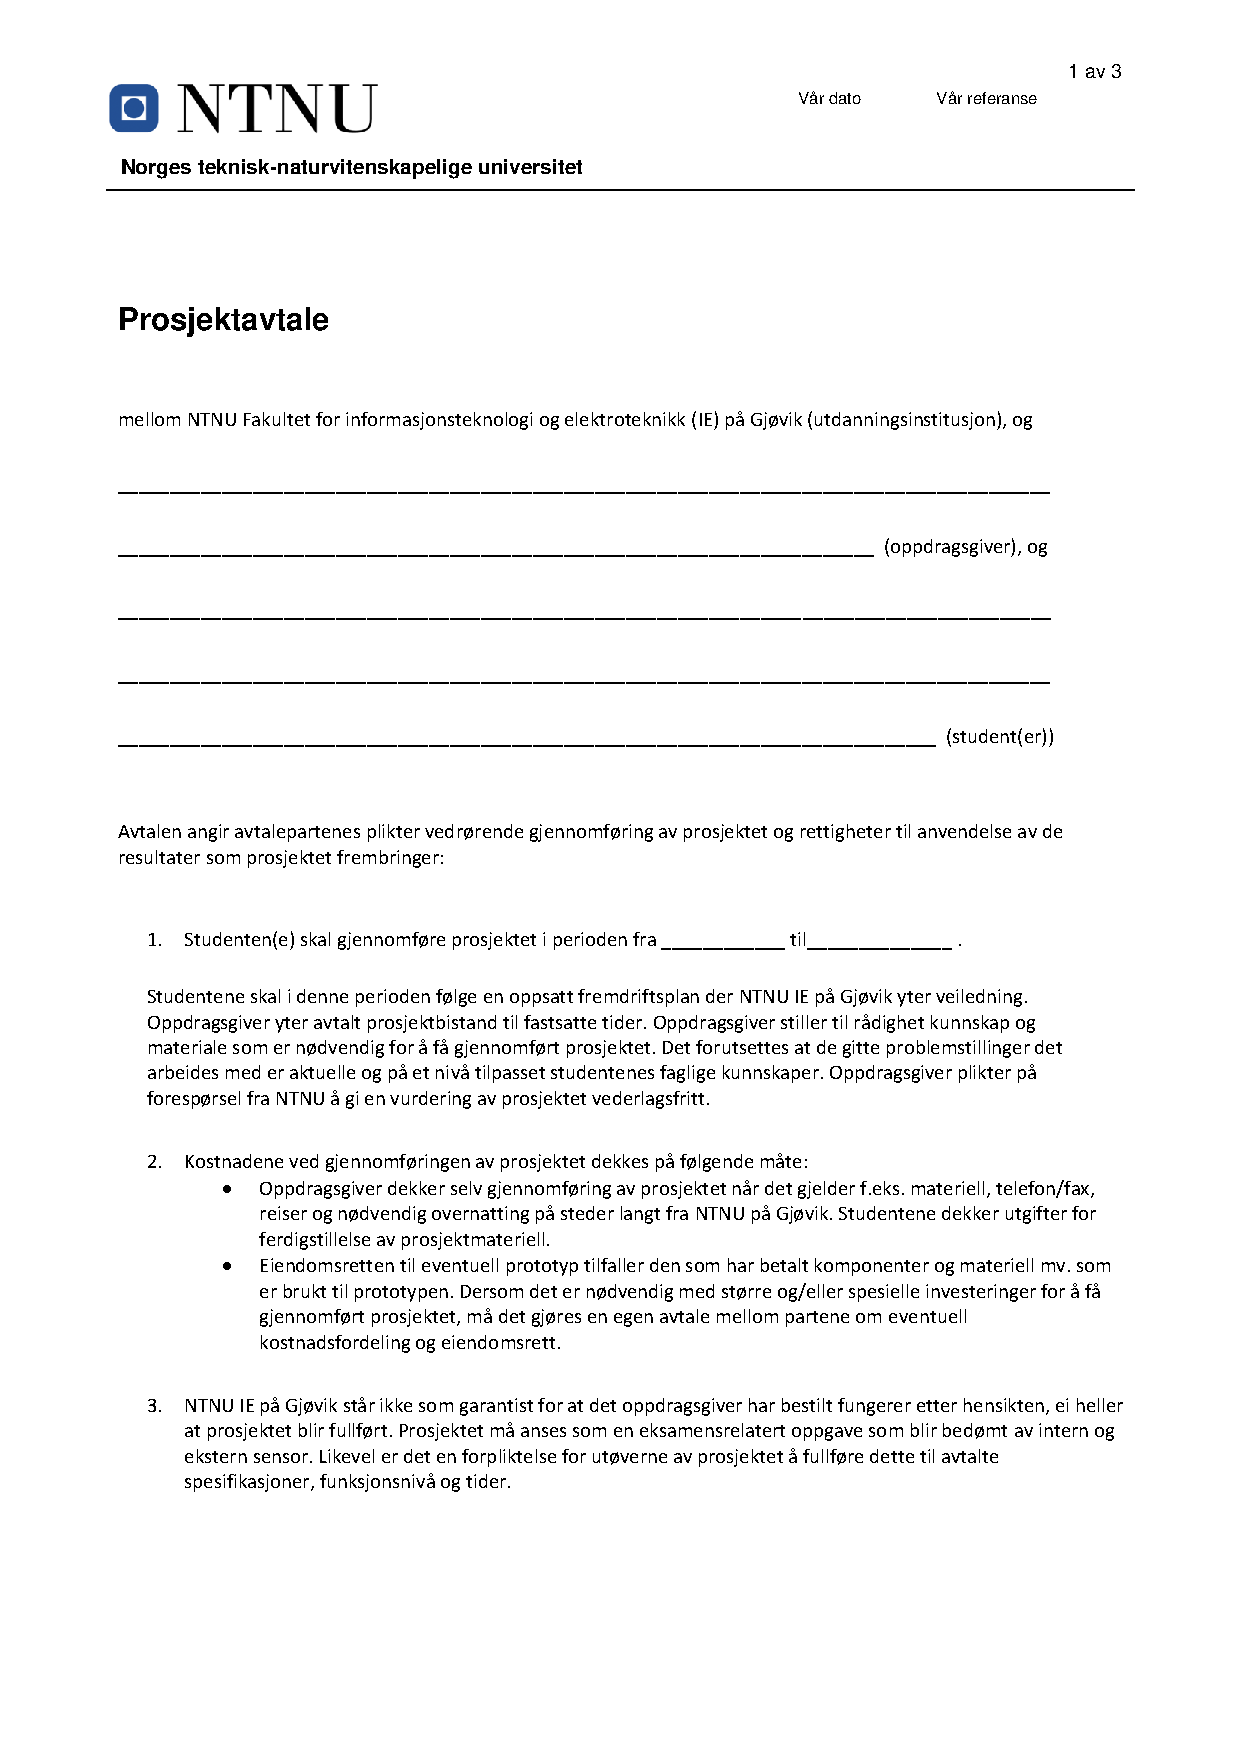
\includepdf[pages=-]{appendices/NTNUProsjektavtale.pdf}

\end{document}
